%%%%%%%%%%%%%%%%%%%%
% Advanced
%%%%%%%%%%%%%%%%%%%%
\section{Advanced}
\begin{codelisting}{advanced_00}{Get an overview of remote branches}
# Get the remote changes
> git fetch
# Show all branches
> git remote show origin
# Show all known branches
> git branch -a
\end{codelisting}
\subsection{Merge conflicts}
On merge conflicts~\mycodelisting{advanced_01} there are mostly three stages of the files involved: "base" 1, "ours" 2 and "theirs" 3 see~\mycodelisting{advanced_02}. Files without merge conflict have only one stage stage namely 0. Sometimes there is no "ours" or no "theirs". That happens when the file is not existent in one repository. Base is the common source of ours and theirs. Ours is the version in the remote repository (github). Theirs is the local version we are working on (the developing server).
\begin{codelisting}{advanced_01}{Merge conflict after pull rebase}
# Not currently on any branch.
# Unmerged paths:
#   (use "git reset HEAD <file>..." to unstage)
#   (use "git add/rm <file>..." as appropriate to mark resolution)
#
#       both modified:    FILE

# NB: during rebase the HEAD got "detached" (see above output)
> git branch
* (no branch)
  master
...
\end{codelisting}
The stages of a file and their content may be displayed as shown in~\mycodelisting{advanced_02} from left to right there are: file permissions, the SHA1, the stage and the filename of the file.
\begin{codelisting}{advanced_02}{List file status}
> git ls-files -s FILE
100755 b42be60e564a0f9a948d08b37fec6ec603793d7e 1       FILE
100755 2c3b3cac7dc0275c073edaae7cee5dd90c90f210 2       FILE
100755 8bf1e221687ce7ec48b180a2f0880239ce34455b 3       FILE
# View the FILE in the different versions
> git show 2c3b3cac7dc0275c073edaae7cee5dd90c90f210 #"ours"
> git show 8bf1e221687ce7ec48b180a2f0880239ce34455b #"theirs"
\end{codelisting}
In~\mycodelisting{advanced_03}/\mycodelisting{advanced_04} we see an example how you can hand merge a file that is stale locally (Home is still present in "their" file) but already has changed in the remote origin (Home has been removed in "our" file).
\begin{codelisting}{advanced_03}{Example of merge conflict}
...
+<<<<<<< Updated upstream                                                                                                                                                                                                                    
    <li class="first-item"><a href=""></a></li>
+=======                                                                                                                                                                                                                                     
+   <li class="first-item"><a href="">Home</a></li>                                                                                                                                                              
+>>>>>>> Stashed changes
...
\end{codelisting}
By editing the file by hand as shown in~\mycodelisting{advanced_04} the preferred version is restored.
\begin{codelisting}{advanced_04}{Example of merge conflict resolved}
...
    <li class="first-item"><a href=""></a></li>
...
\end{codelisting}
Alternatively, because obviously "our" file is needed, that version may be fetched as shown in~\mycodelisting{advanced_05}.
\begin{codelisting}{advanced_05}{Example of merge conflict resolved alternative}
> git checkout --ours FILE
\end{codelisting}
In another example a merge conflict has happened in on of the following files: .htaccess, db\_script, robots.txt or typo3conf/localconf.php~\mycodelisting{console_output_00}. In order to keep the version that is running on the developing server and discard remote changes \texttt{git checkout --theirs FILE} is used.
\subsubsection{Mergetool}
After solving the conflicts or as a conflict resolution mergetool is run. Basically when started it needs some resolution tool. The default can be set in the .gitconfig file in the users home directory. In~\myfigure{fig:diff_view00} a typical resolution Situation is shown.
\label{fig:diff_view00}
\begin{figure}[htbp]
  \centering
  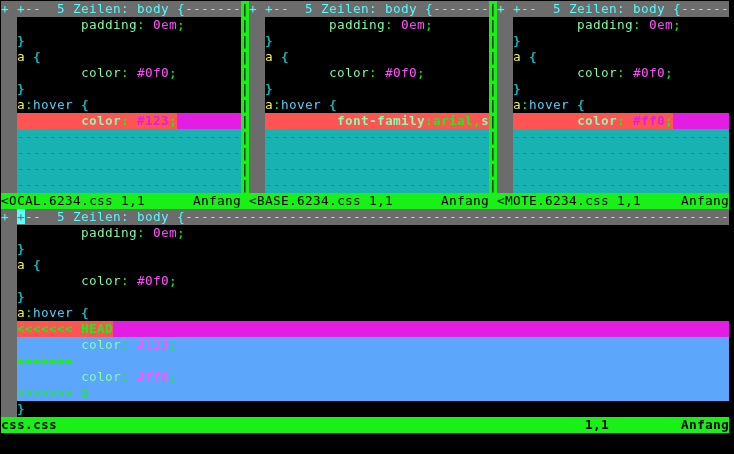
\includegraphics[width=\textwidth]{vimdiff_mergetool_00.png}
  \caption{Diff view with base, ours, theirs and current file}
\end{figure}

The~\myfigure{fig:diff_view01} shows the situation after the local file has been edited. Saving the file and quitting all buffers will tell git the merge was successful.
\label{fig:diff_view01}
\begin{figure}[htbp]
  \centering
  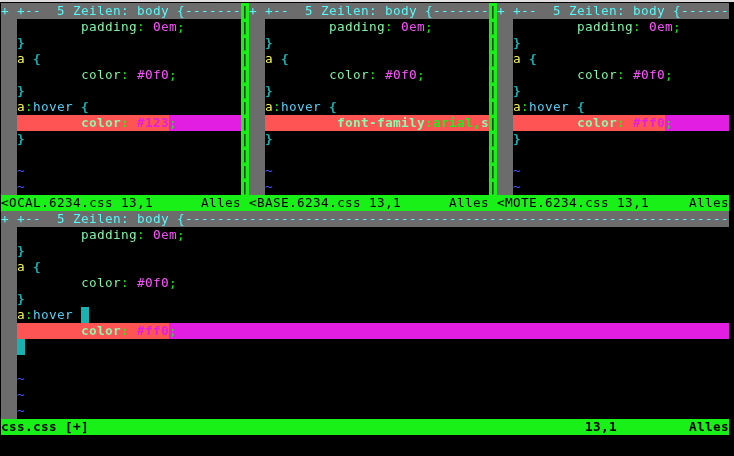
\includegraphics[width=\textwidth]{vimdiff_mergetool_01.png}
  \caption{Edited the file}
\end{figure}

If ours or theirs was checked out beforehand and the file therefore is not saved in editor vimdiff git asks you to confirm the merge success as shown in \mycodelisting{advanced_06}.
\begin{codelisting}{advanced_06}{Closed the editor without saving}
>git mergetool
Merging:
css.css

Normal merge conflict for 'css.css':
  {local}: modified
  {remote}: modified
Hit return to start merge resolution tool (vimdiff): 
4 Dateien zum Editieren
css.css seems unchanged.
Was the merge successful? [y/n]
\end{codelisting}
\subsection{Finding branches knowing the commit SHA1}
\begin{codelisting}{advanced_07}{Finding branches knowing the commit SHA1}
> git branch --contains 864afa58a82c58e4367ac4e2b70b57d667494a8c
* master
> git branch -r --contains 0fc352ba9abea4d9ec8e
  origin/werksfarbe_0008632_umbau_der_tabs_auf_first_child
\end{codelisting}
\subsection{Config file}
Use the \texttt{help config} command to find out about all the settings.
\begin{codelisting}{advanced_08}{Configuring git}
> git config --global user.name 'Patrick-Emil Zoerner'
> git config --global user.email 'zoerner@vsp.ag'
> git config --global github.user paddyez
> git config --global github.token 0123456789yourf0123456789token
# Colors for black background and green as font color
> git config --global color.branch.current 'yellow bold'
> git config --global color.branch.remote 'cyan bold'
> git config --global color.diff.new 'yellow bold'
> git config --global color.diff.old 'red bold'
> git config --global color.diff.meta 'cyan bold'
> git config --global color.diff.frag 'white bold'
> git config --global color.diff.commit 'white bold'
> git config --global color.status.added 'yellow bold'
> git config --global color.status.changed 'cyan bold'
> git config --global color.status.untracked 'red bold'
\end{codelisting}
Alternatively and if you know what you are doing you can edit the file .gitconfig.
\begin{codelisting}{advanced_09}{.gitconfig}
[user]
        name = Patrick-Emil Zoerner
        email = zoerner@vsp.ag
[github]
        user = paddyez
        token = 0123456789yourf0123456789token
[merge]
        tool = vimdiff
[diff]
        color = auto
[alias]
        st = status
        ci = commit
        co = checkout
        br = branch
        di = diff --ignore-all-space
[color "branch"]
        current = yellow bold
        remote = cyan bold
[color "diff"]
        new = yellow bold
        old = red bold
        meta = cyan bold
        frag = white bold
        commit = white bold
[color "status"]
        added = yellow bold
        changed = cyan bold
        untracked = red bold
\end{codelisting}
\subsection{Make non git repository a git repository}
\begin{codelisting}{advanced_10}{}
git init
git remote add origin git://git/vsp.ag
git pull --rebase origin master
\end{codelisting}
\subsection{Install a git public repository on debian}
\begin{codelisting}{advanced_11}{Installing }
> sudo apt-get install git-core gitweb
> sudo mkdir /var/www/git 
> [ -d "/var/cache/git" ] || sudo mkdir /var/cache/git
> sudo vim /etc/apache2/sites-available/git
--8<--
<VirtualHost *:80>
        ServerName      git
        DocumentRoot    /var/www/git/
        <Directory /var/www/git>
                Allow from all
                AllowOverride all
                Order allow,deny
                Options ExecCGI
                <Files gitweb.cgi>
                        SetHandler cgi-script
                </Files>
        </Directory>
        DirectoryIndex gitweb.cgi
        SetEnv  GITWEB_CONFIG  /etc/gitweb.conf

        CustomLog       /var/log/apache2/git_access.log combined
        ErrorLog        /var/log/apache2/git_error.log
        RewriteLog      /var/log/apache2/git_rewrite.log
        RewriteLogLevel 3
</VirtualHost>
-->8--
> sudo a2ensite git
> sudo cp /usr/share/gitweb/* /var/www/git
> sudo cp /usr/lib/cgi-bin/gitweb.cgi /var/www/git
> cd /var/www/git
> ln -s /usr/lib/cgi-bin/gitweb.cgi index.cgi
> sudo vim /etc/gitweb.conf
--8<--
# path to git projects (<project>.git)
$projectroot = "/var/cache/git";
# directory to use for temp files
$git_temp = "/tmp";
# target of the home link on top of all pages
#$home_link = $my_uri || "/";
# html text to include at home page
$home_text = "indextext.html";
# file with project list; by default, simply scan the projectroot dir.
$projects_list = $projectroot;
# stylesheet to use
$stylesheet = "gitweb.css";
# logo to use
$logo = "git-logo.png";
# the 'favicon'
$favicon = "git-favicon.png";
-->8--
> sudo etc/init.d/apache2 reload
> cd /var/cache/git/
> mkdir vsp.ag
> cd vsp.ag
> git init
> git config --bool core.bare true
> echo "VSP AG & Fondsvermittlung24.de" > .git/description
> git commit -a
> touch .git/git-daemon-export-ok
> git daemon --base-path=/var/cache/git --detach --syslog --export-all --enable=receive-pack
> git clone git://git/vsp.ag vsp.ag 
\end{codelisting}